\section{Design analysis and concept diagrams}
Description of issues related to the design of the product:
- Description of concepts, requirements and features of the product
- Review of motivations for making the design decisions
- Indicate the primary features of the design that are the most creative and original

\subsection{Materials}
For this project we got a bunch of different plast materials from RIAS, in order to find some material that might be cheaper, and better that acrylic, since acrylic have tendency to be brittle, this becomes worse when it has been laser cut.
all of the plastic was thermoplastic, which is a term that is used in the laser industri to indicate that it can be laser c ut.
for the laser cutter we made some simple figures to see what the result would be.
\subsubsection{PEHD}
The first material that we tryed to cut was, PEHD which is used in the production of ex. plastic bottles and corrosion-resistant piping it is know for having a high strength to density ratio.
The cutting went fine, but there was some resedu left over from the cutting, that we had some problems removing.
% There ware some problems getting the resedu off the plastic after the cutting, also the material have a tendensy to hold it's form when bent.%
\begin{figure}[h]
	\begin{center}
		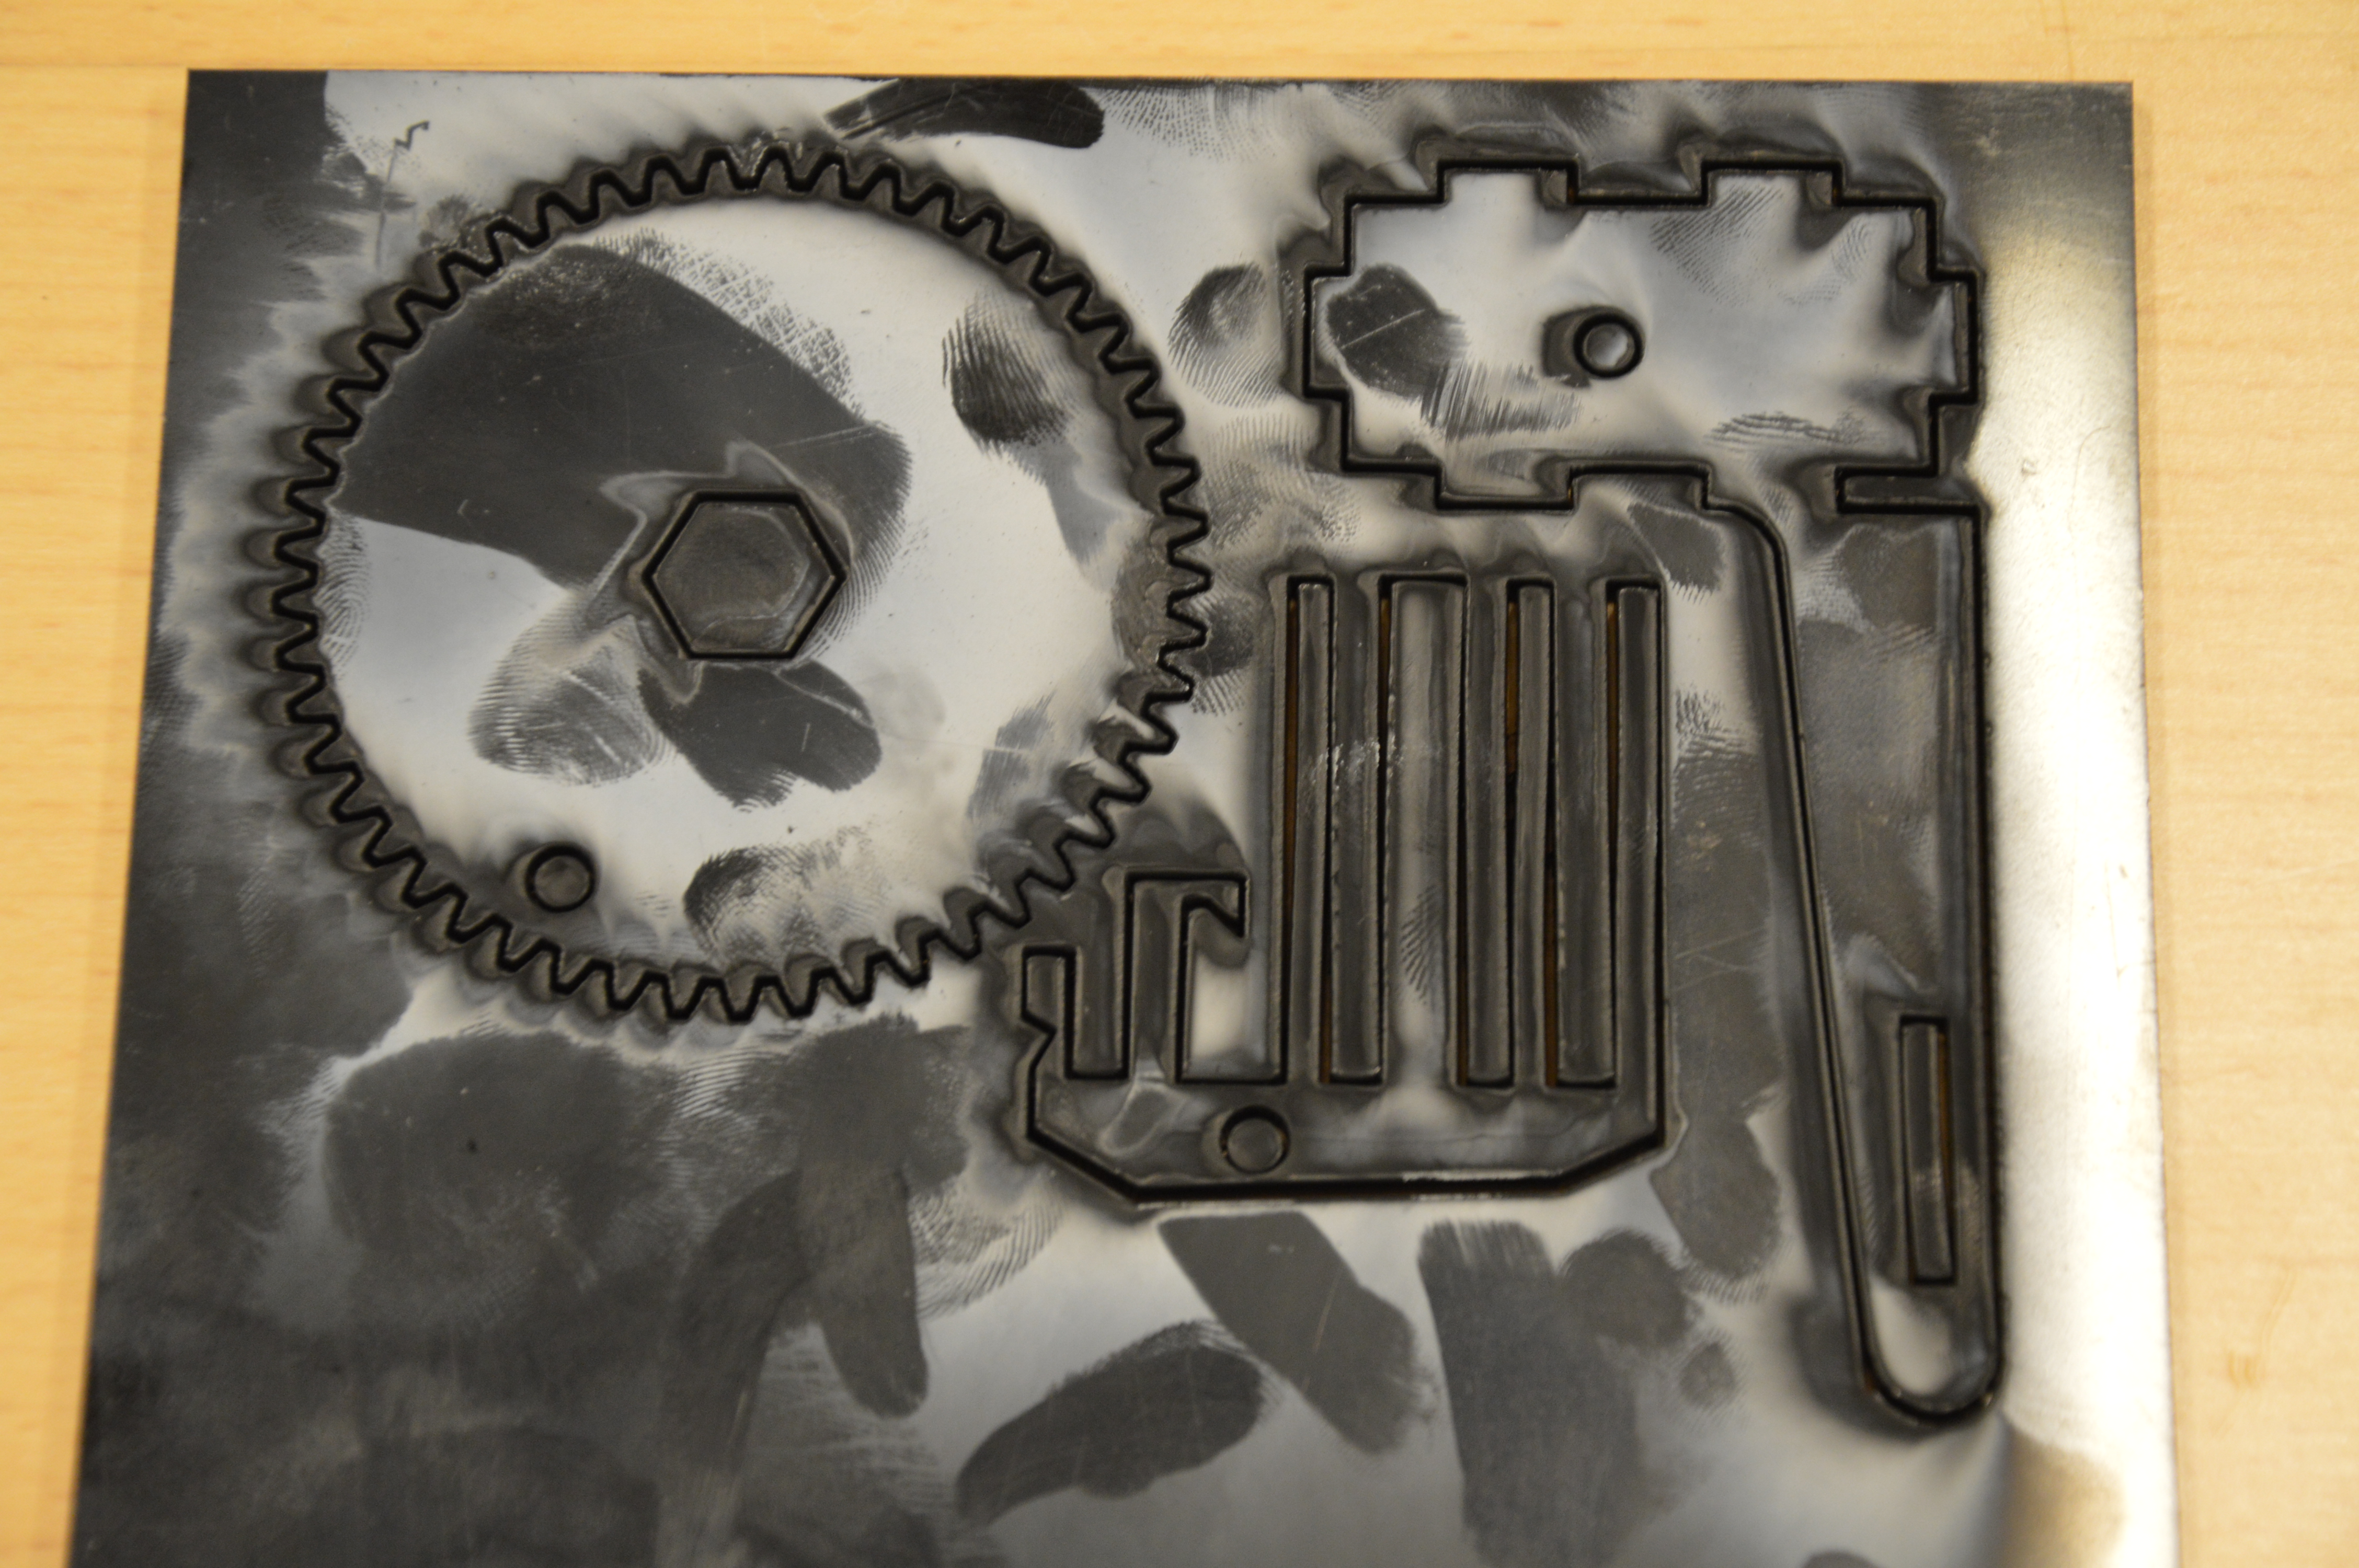
\includegraphics[scale=0.1]{images/DSC_0048.JPG}
		\caption{\small {\it {Cut test of PEHD}}} \label{fig:explode}
	\end{center}
\end{figure}
\subsubsection{ PP}
RIALEN PP  is most commenly used in packaging and labeling, and it has resistant to many chemical solvents, bases and acids.
The cuttig had some big problems, one of them was that after 3 cutting rounds, the laser still haven't cut through the material, which ment we had to let it be, and not trying to cut in that material. 
\begin{figure}[h]
	\begin{center}
		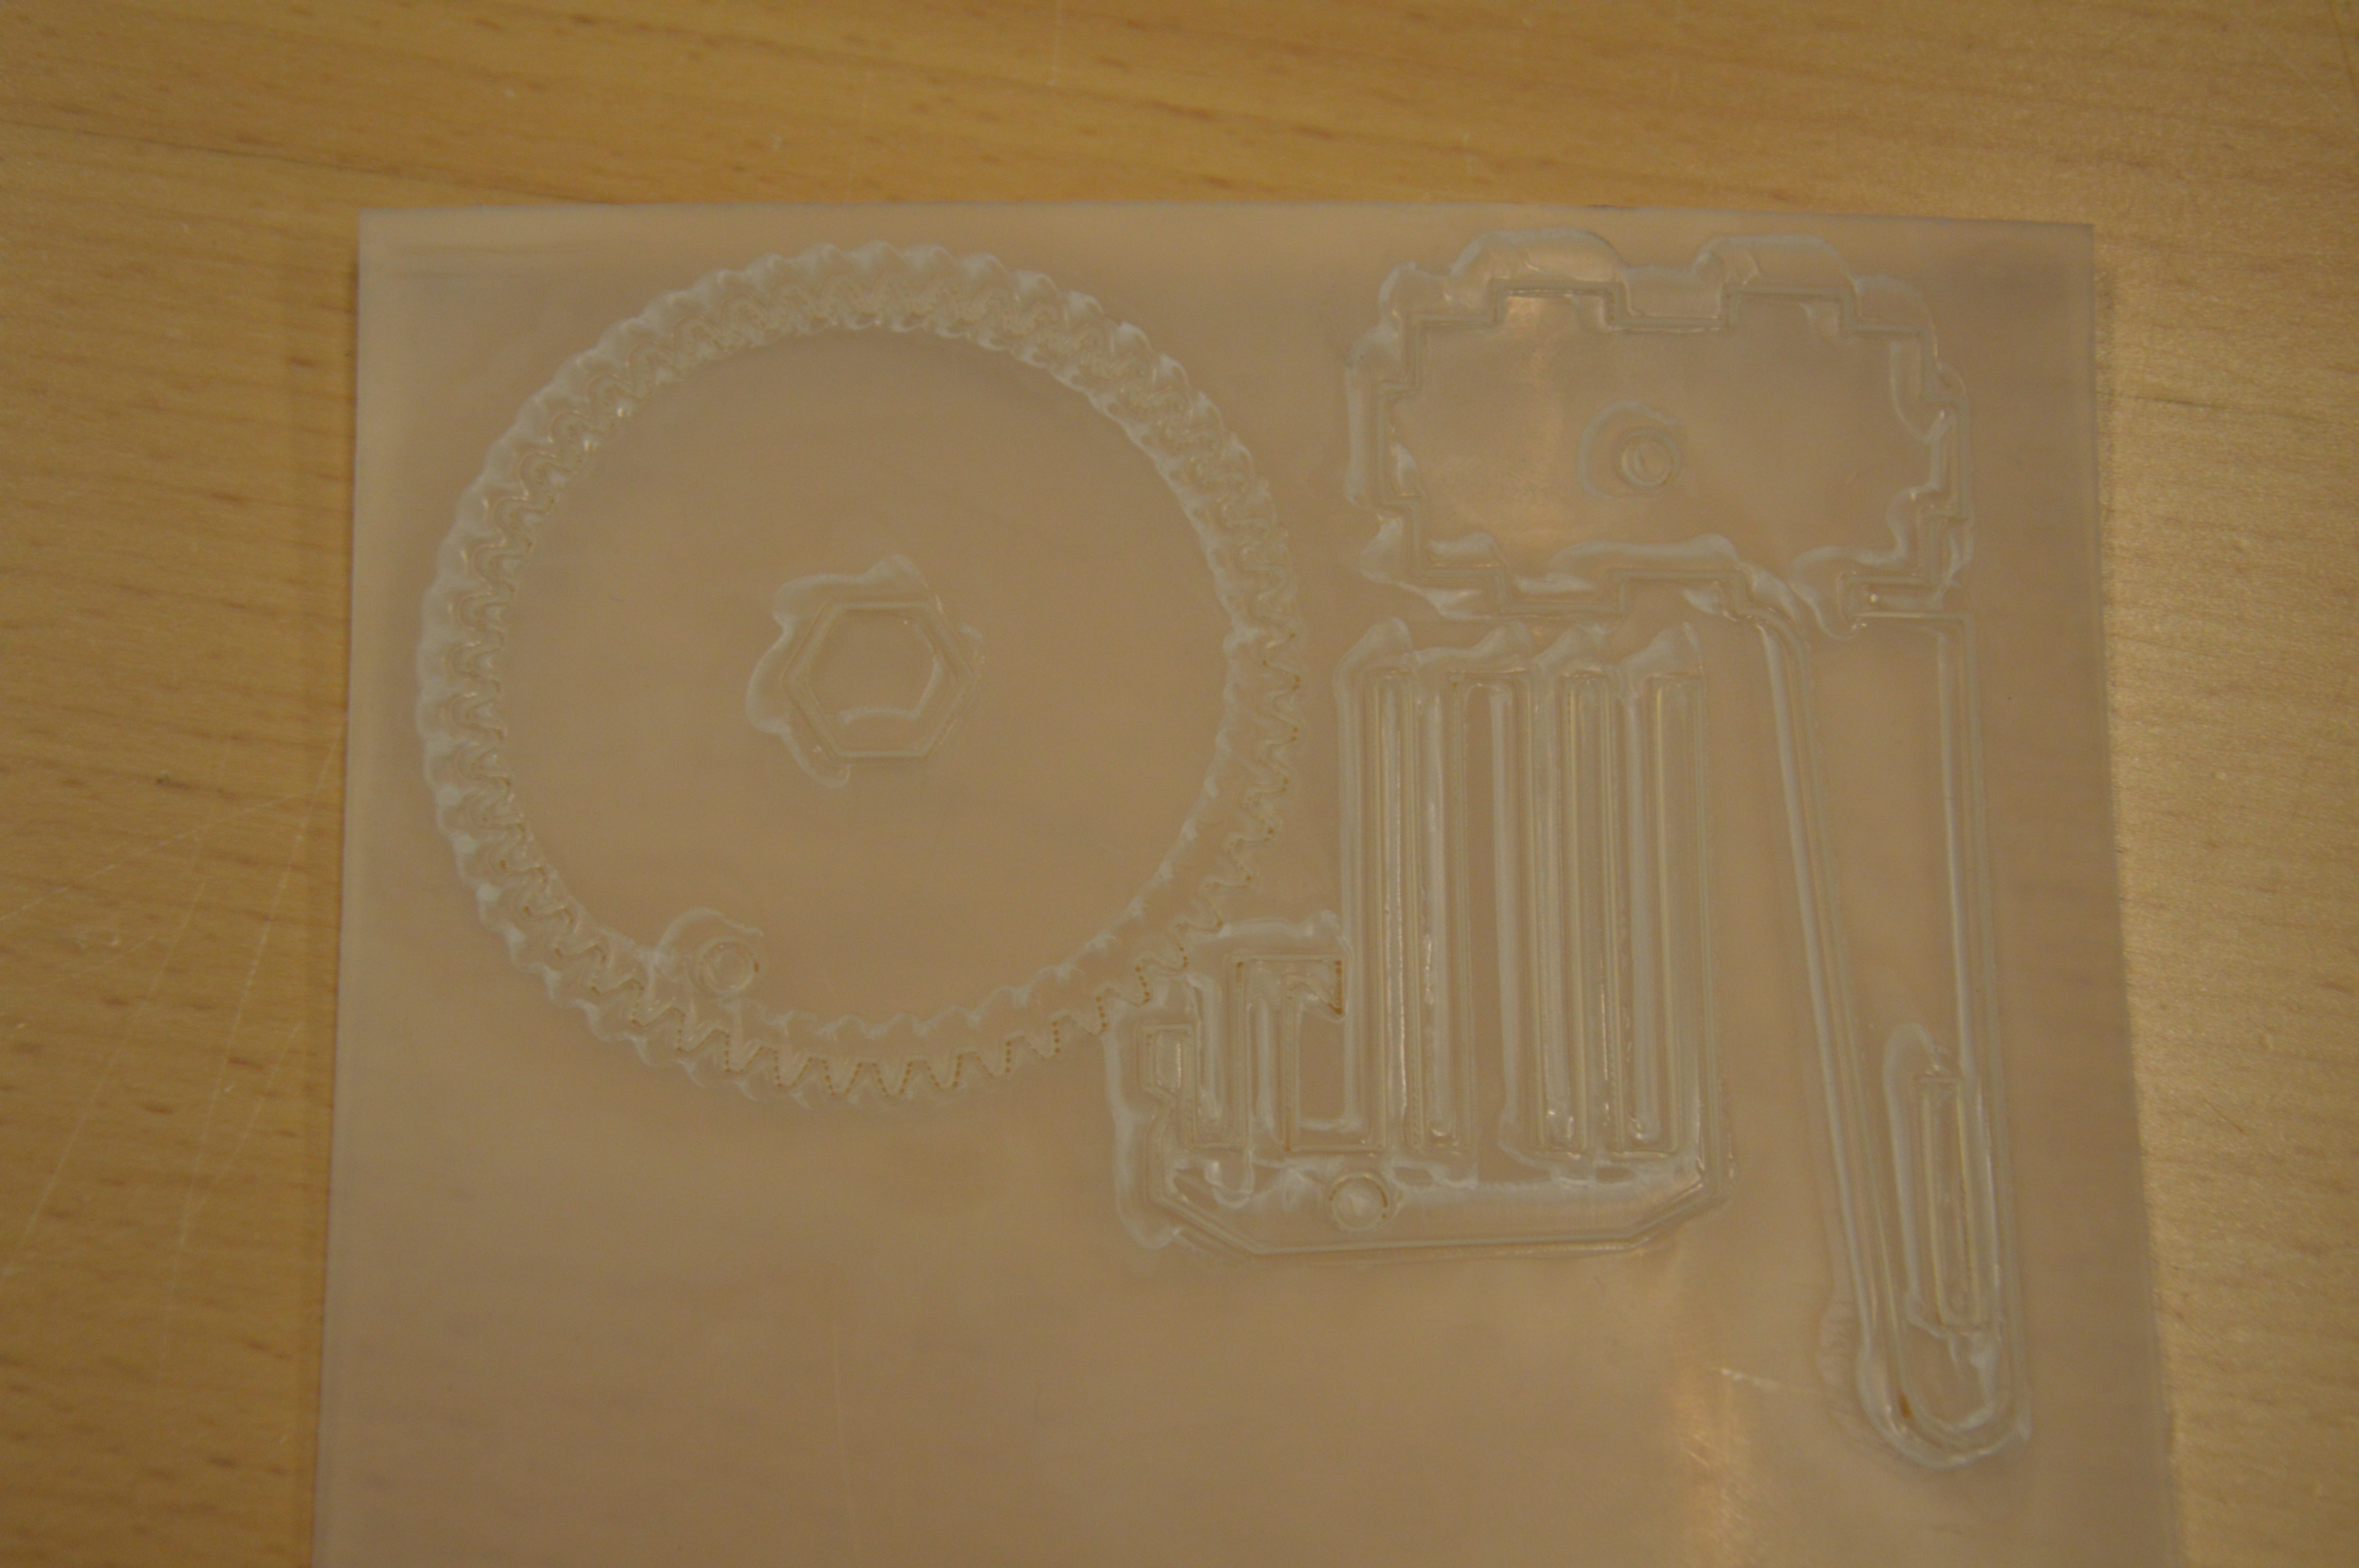
\includegraphics[scale=0.1]{images/DSC_0053.JPG}
		\caption{\small {\it {Cut of RIALEN PP}}} \label{fig:explode}
	\end{center}
\end{figure}
\subsubsection{PP-H}
Is PP where they have added Homopolymer ot, this changes the material, so it is becomes easyer to cut, but it leaves some resudey, when cut, it also have tendensy to curle up, on it self.
One of the things that arent good with the material is that it is flexible and keeps it shape, when bent, which means that it canøt be used for the patient record. 
\begin{figure}[h]
	\begin{center}
		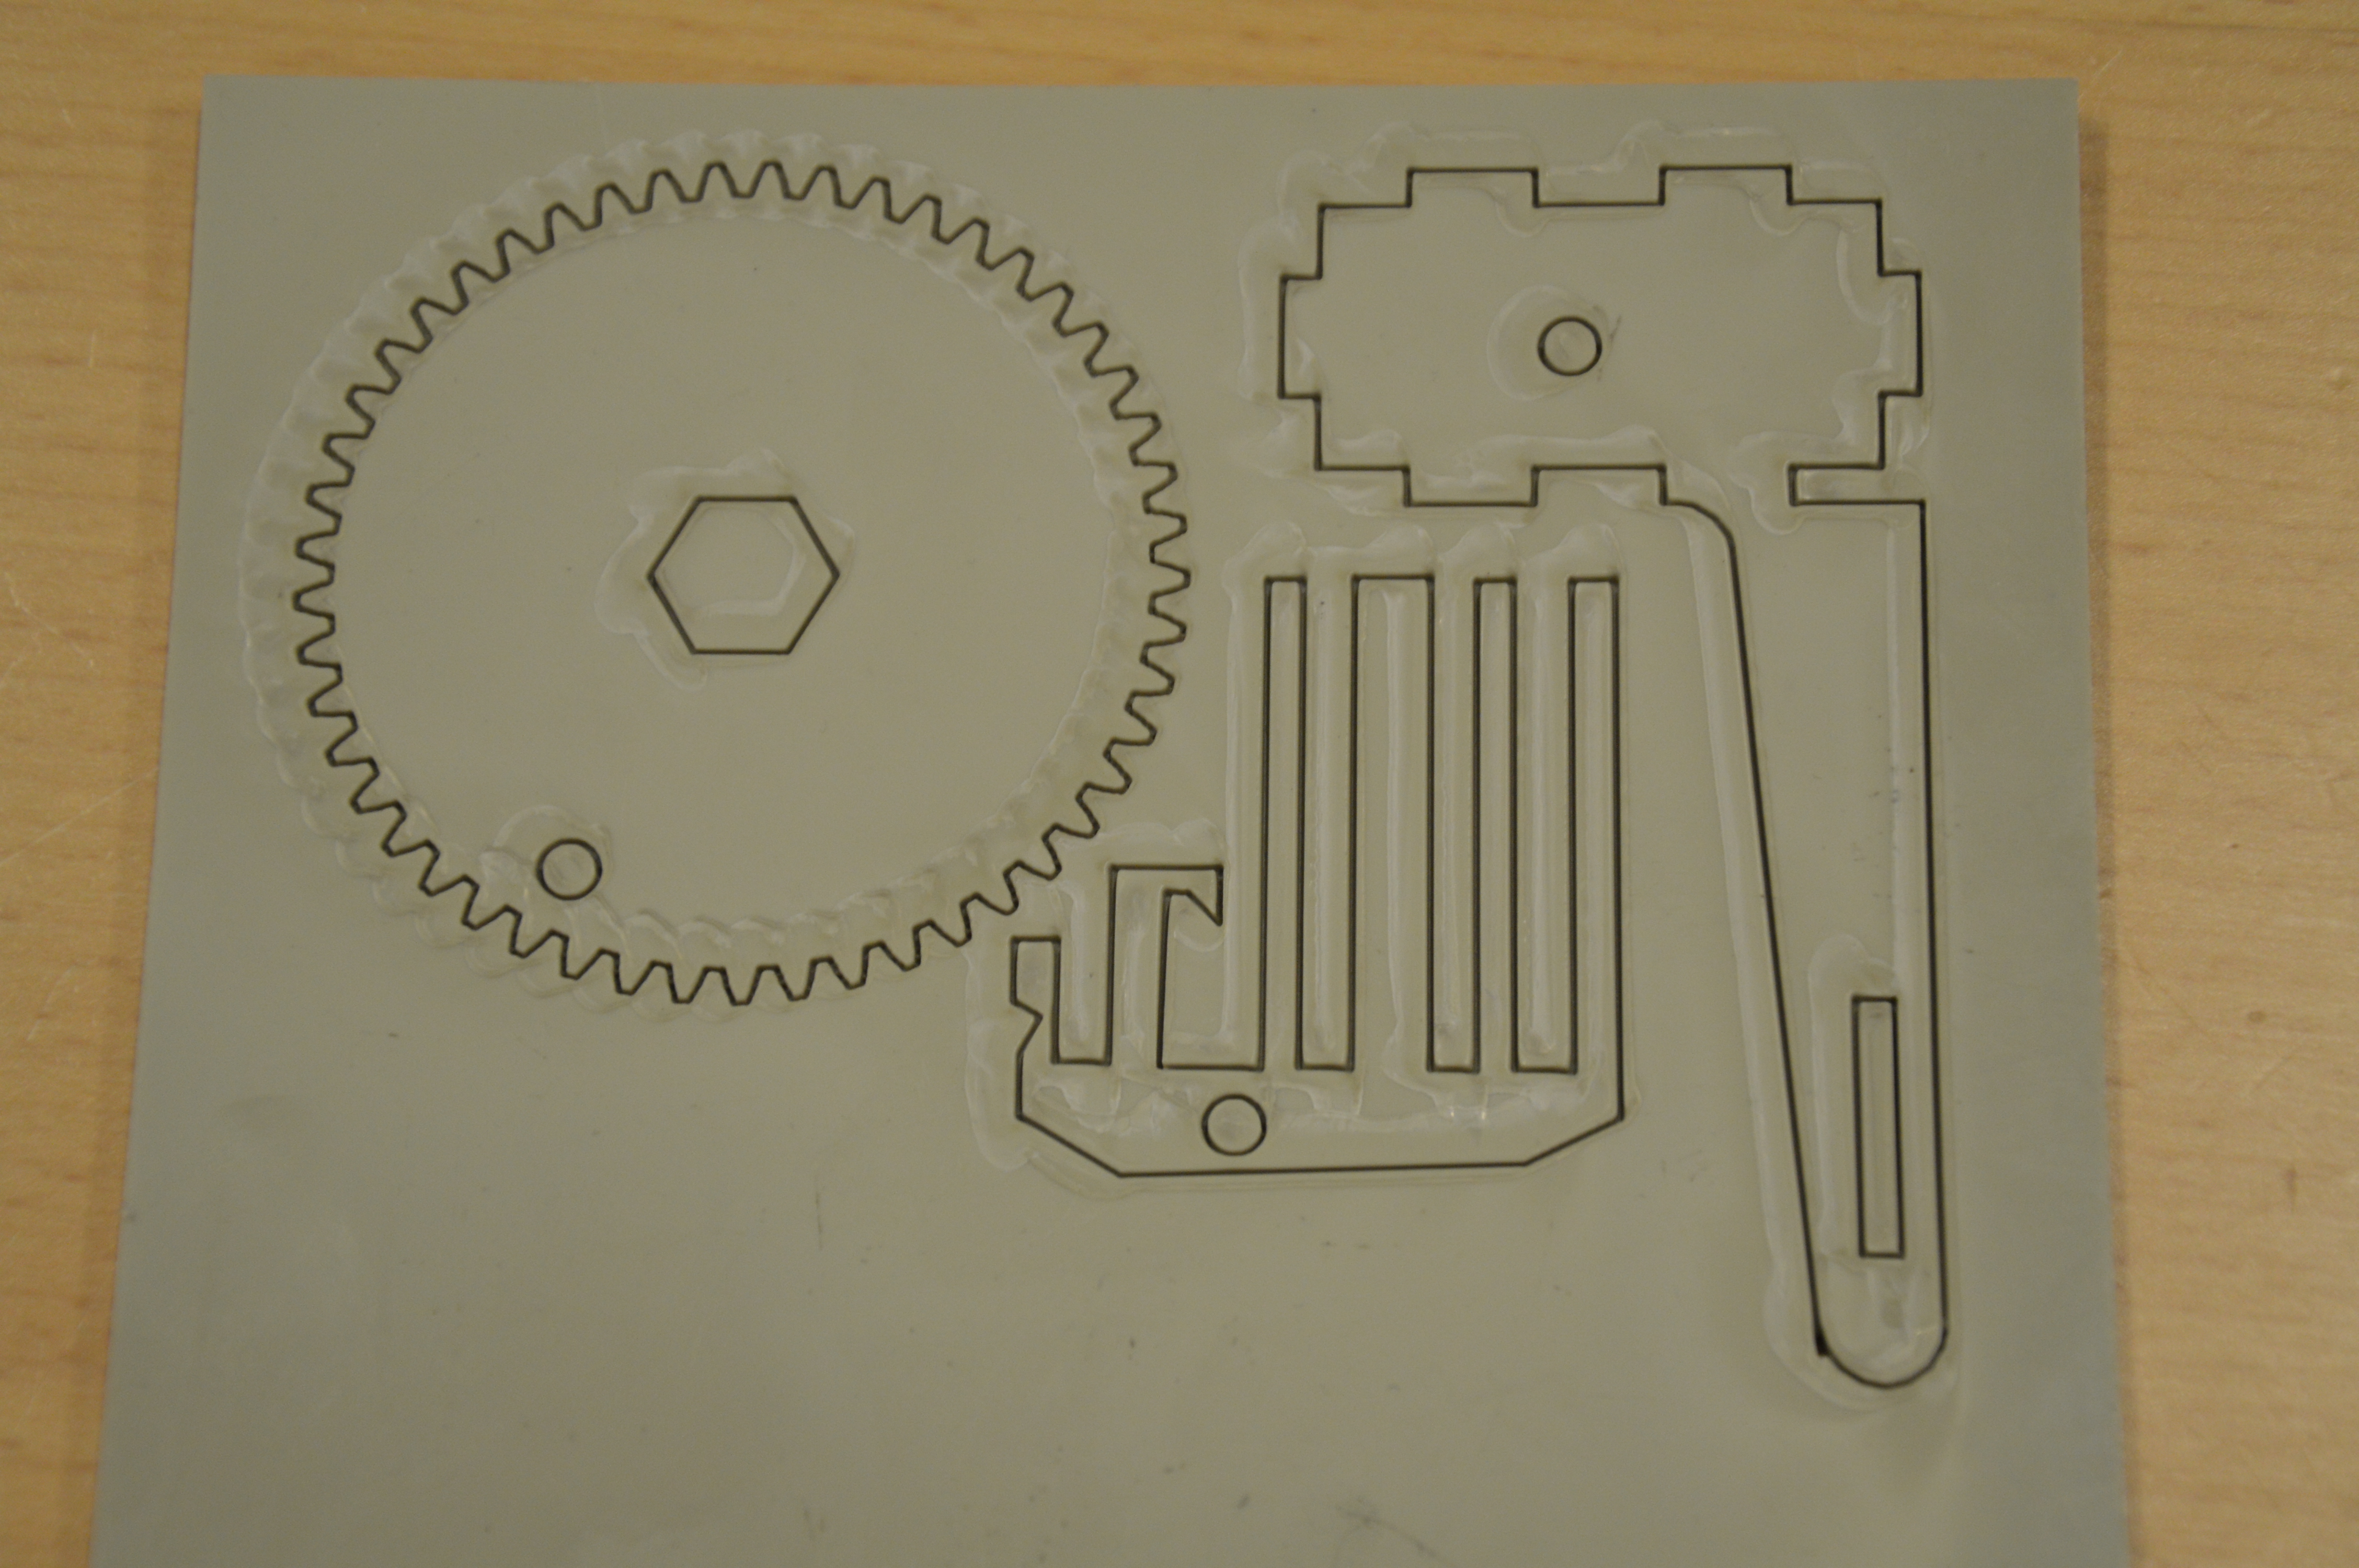
\includegraphics[scale=0.1]{images/DSC_0029.JPG}
		\caption{\small {\it {Cut test of PP-H}}} \label{fig:explode}
	\end{center}
\end{figure}

\subsubsection{PETG}
PETG is used alot in the production of plastic bottles, and is a durable material.
The cutting process did not go as hopede, be side that one can see the burn marks, it also had a very strong cemical smell, that took a log time to disapate.
\begin{figure}[h]
	\begin{center}
		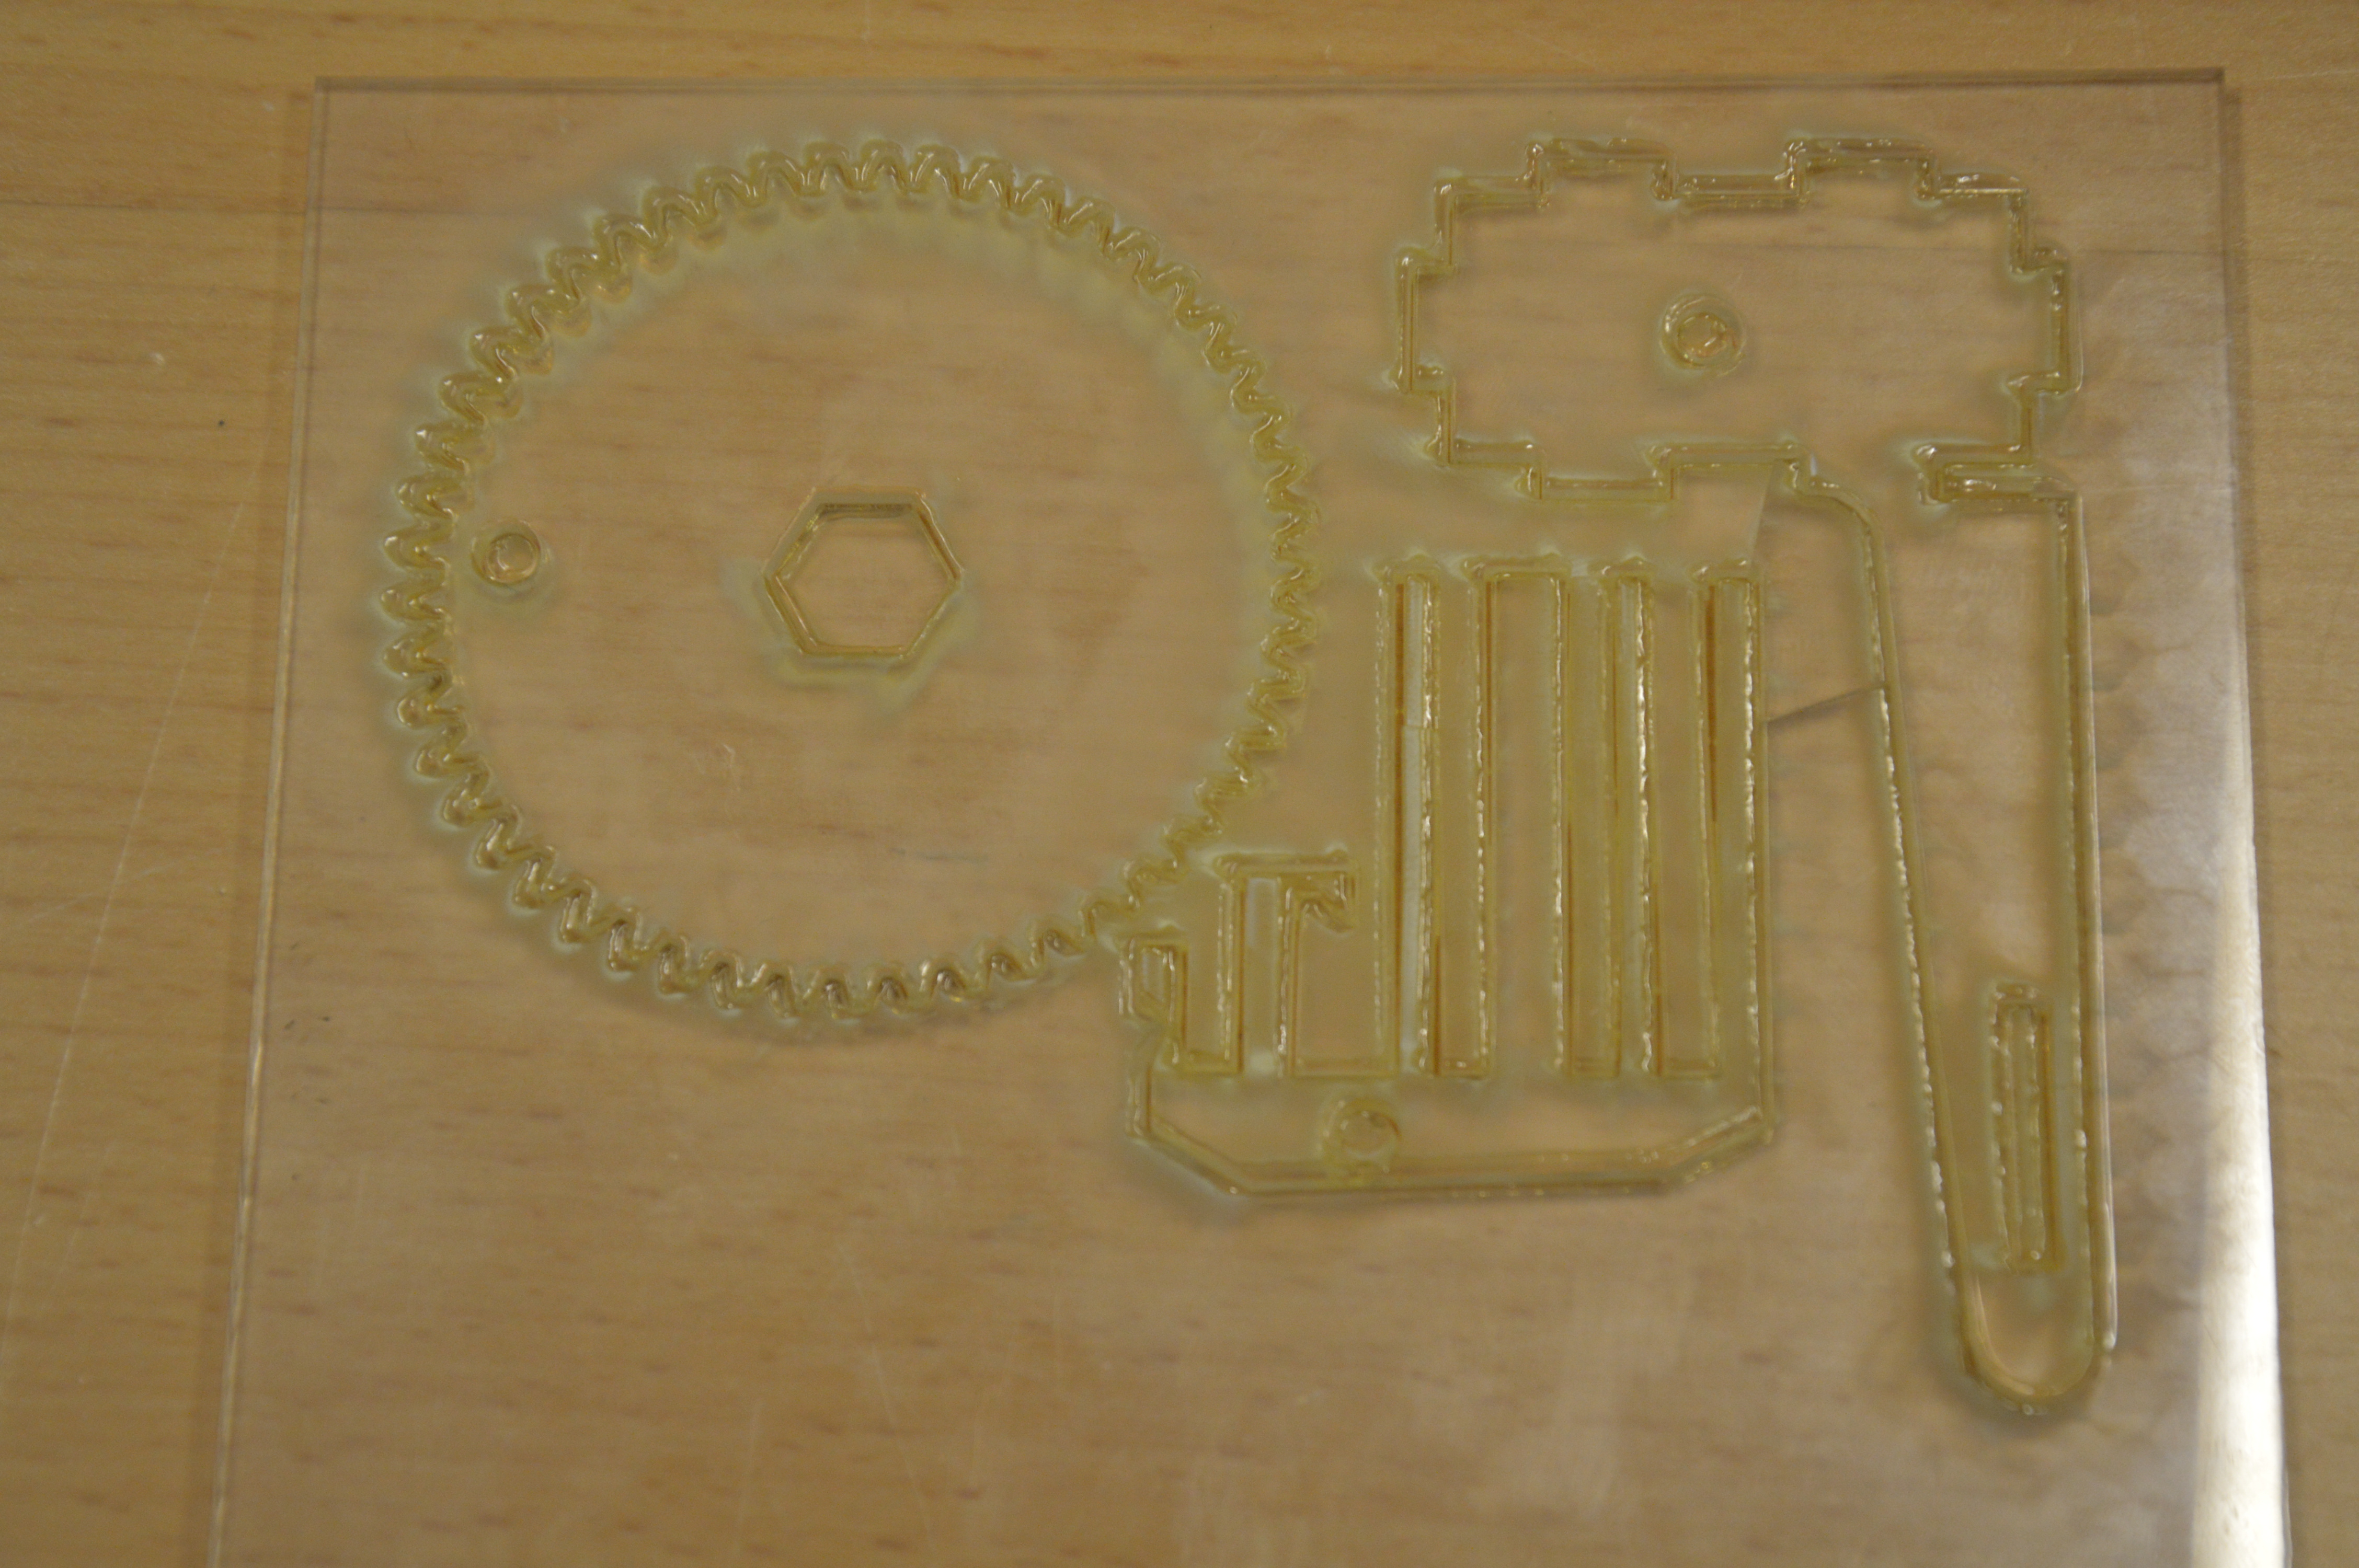
\includegraphics[scale=0.1]{images/DSC_0023.JPG}
		\caption{\small {\it {Cut test of PETG}}} \label{fig:explode}
	\end{center}
\end{figure}
\subsubsection{POM-C}
POM-C is a material that works well with laser cutting, it is used commenly in small gear wheels, ball bearings, and many othere product where you need low friction and stifness.
The cutting of it went fine, but we found out that if we want to use it, we may have some problems since the glue, that is used for it is highly toxic, futhere more the material is expensive compaired to Acrylic
\begin{figure}[h]
	\begin{center}
		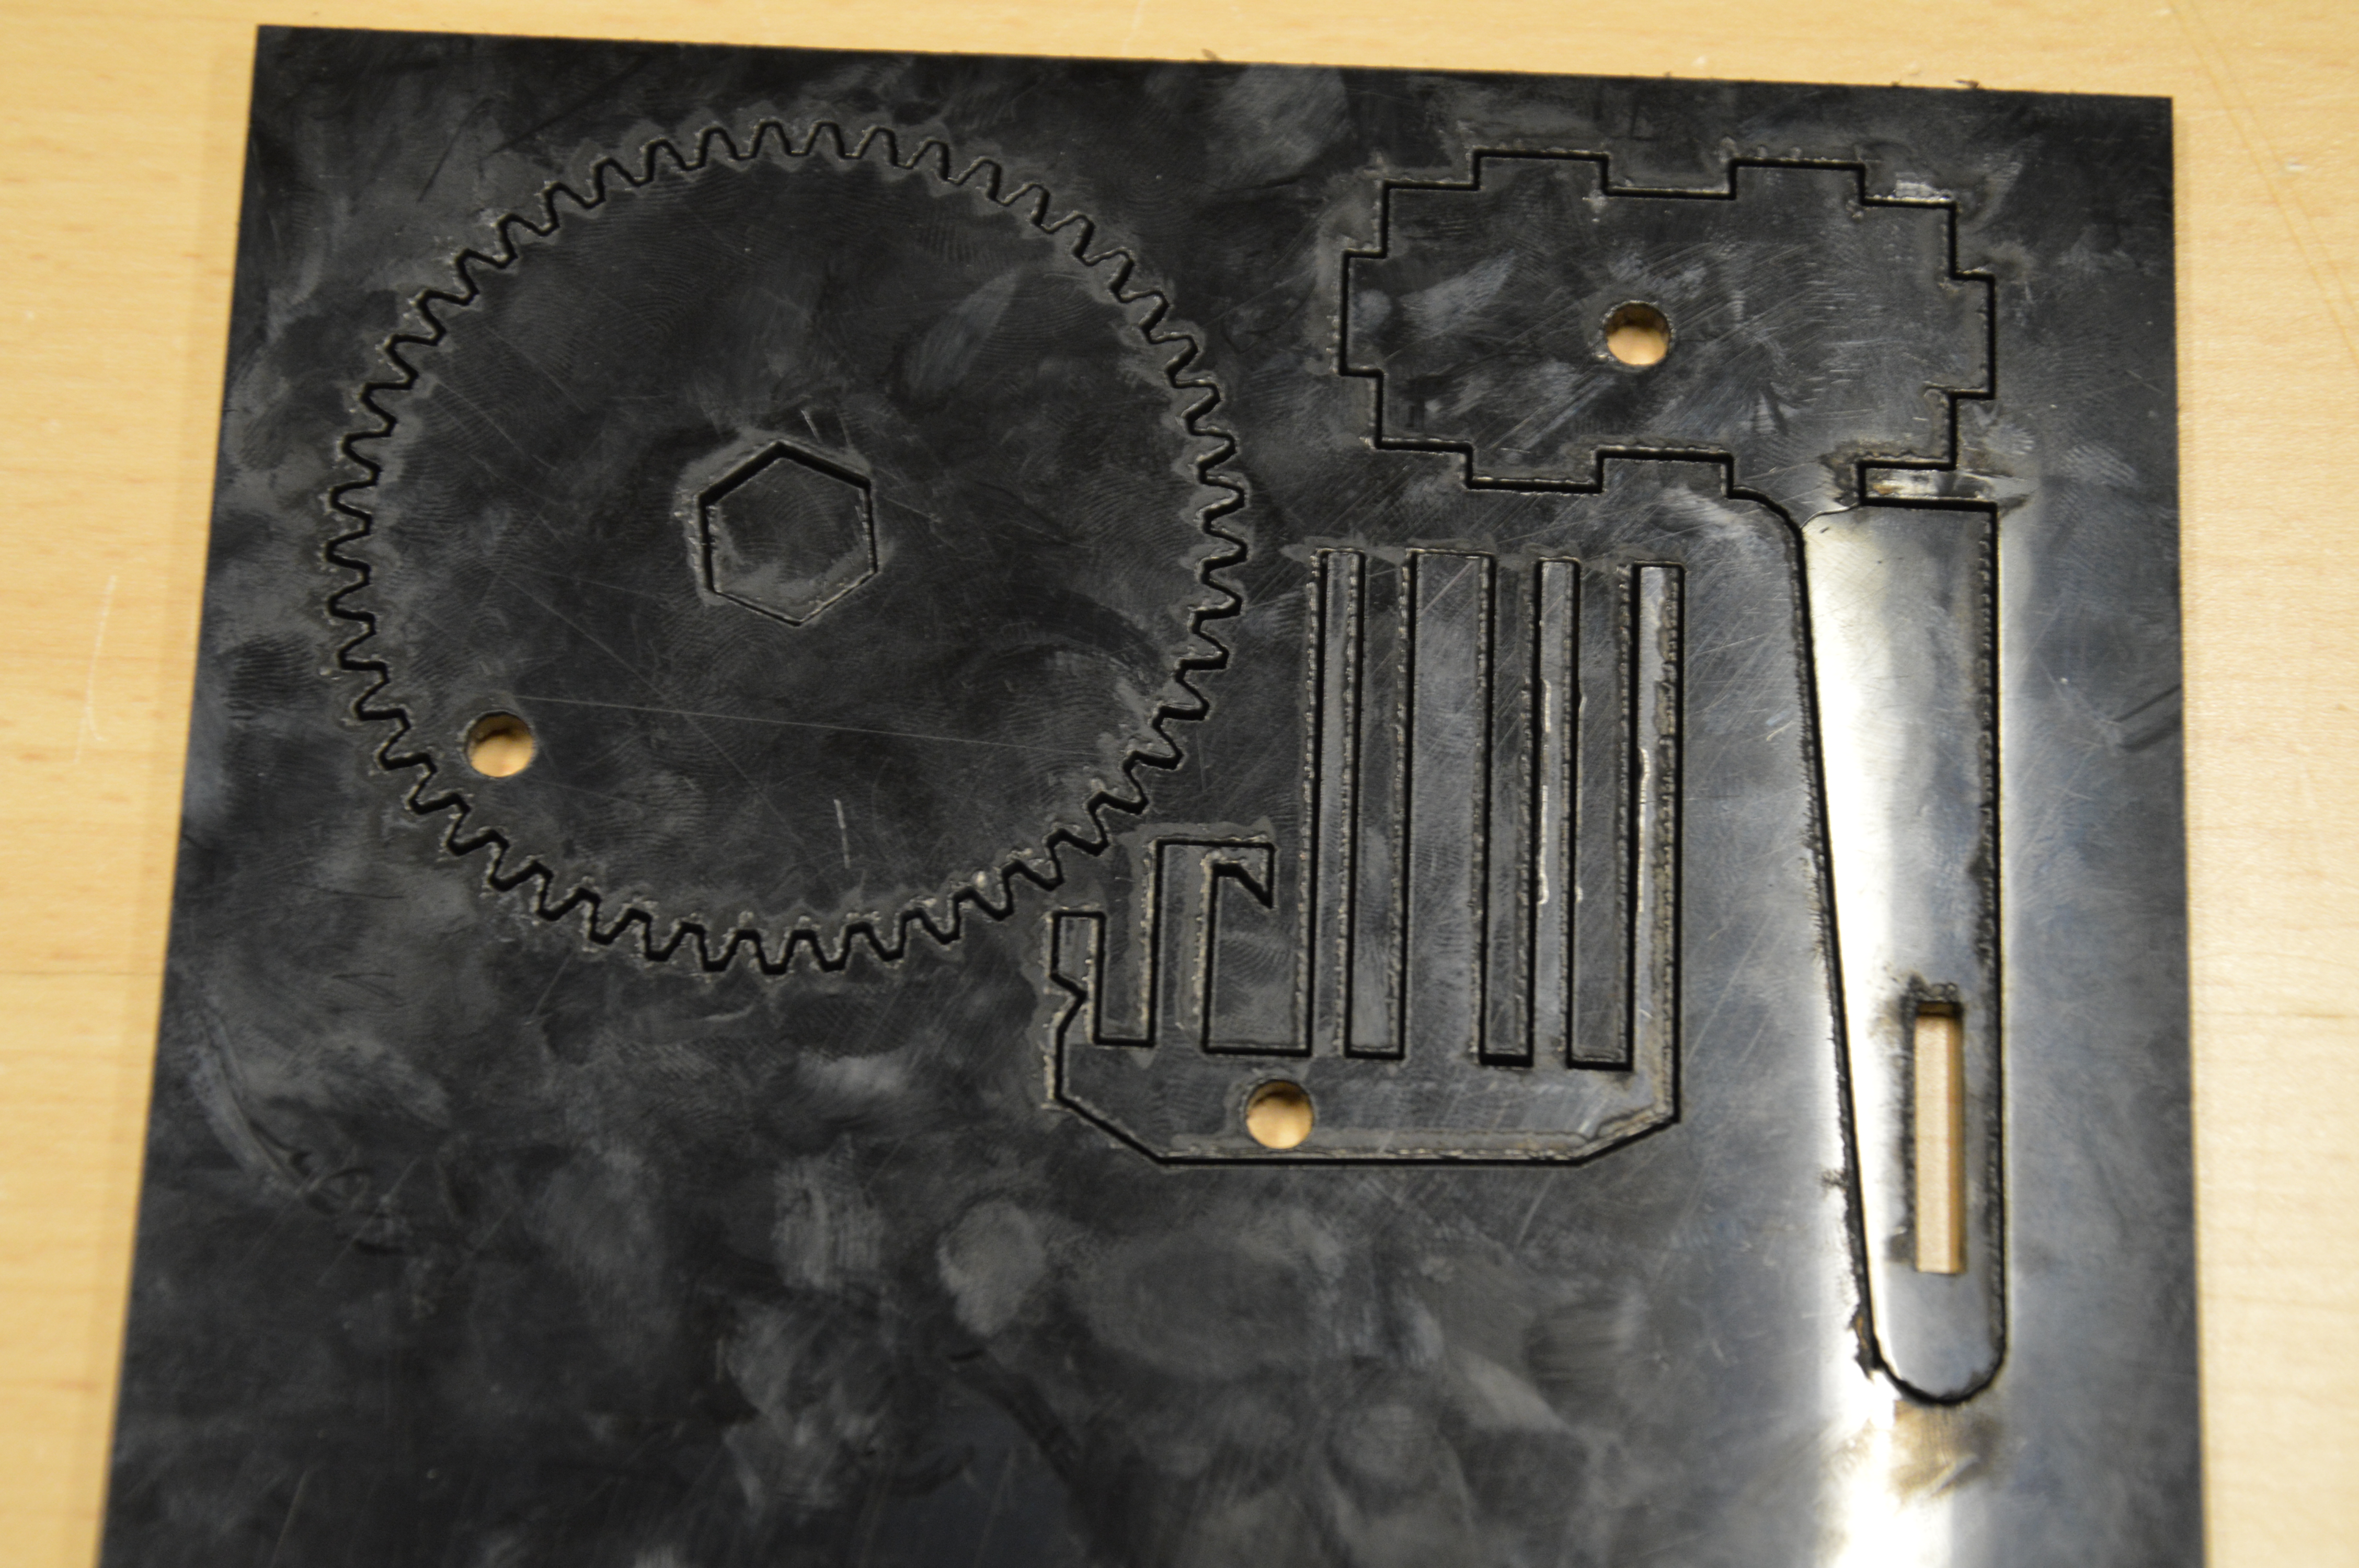
\includegraphics[scale=0.1]{images/DSC_0039.JPG}
		\caption{\small {\it {Cut test of POM-C}}} \label{fig:explode}
	\end{center}
\end{figure}

\subsubsection{PEEK}
PEEK is one of the materials that we whould have liked to try out since it is one of the materials that are used in the me dical industry, however it is an expensive material and it is had to get, we did have some conversion over mail with RIAS, but was unable to secure some samples.

\subsubsection{ACRYL}

\subsubsection{Conslusion}

\subsection{Iterations}
we have used prototyping in order to get a viable device, through the different designs we have been able to see different problems, which have ment that we had to iterate to a new version, we have been limited by time, so we have had to make some compromises

\subsubsection{fisrt}
The first iteration that we build did have some problems.
The first is that it is expensive to build, since we are using a lot of acrylic, the secound point is that it still is heavy, and unwieldy.
But i did give some ideas for the next iteration.

\subsubsection{secound}


\subsubsection{thried}


\subsubsection{fourth}


\subsubsection{fith}

\subsubsection{sixth}

